\documentclass[11pt,a4paper]{article}

\usepackage{geometry}
\geometry{margin=1in}

\usepackage{amsmath,amssymb,amsfonts}
\usepackage{graphicx}
\usepackage{textcomp}
\usepackage{xcolor}
\usepackage{booktabs}
\usepackage[T1]{fontenc}
\usepackage{hyperref}

\usepackage{tikz}
\usetikzlibrary{positioning}
\usepackage{pgfplots}
\pgfplotsset{compat=1.18}




\hypersetup{
    colorlinks=true,
    linkcolor=blue,
    citecolor=blue,
    urlcolor=blue
}

\begin{document}

{An SAP-Oriented Predictive Decision Framework for Logistics Risk Monitoring Using Machine Learning and Human-in-the-Loop Control
}

\author{
Author 1, Author 2 }



\maketitle

\begin

\begin{abstract}

Traditional statistical process control and enterprise systems are predominantly retrospective, limiting their ability to support proactive operational intervention. This study presents an SAP-oriented predictive decision framework that connects large-scale logistics transaction data with supervised machine learning, probabilistic risk estimation, human-in-the-loop decision control, SAP-oriented workflow simulation, and cost-sensitive economic evaluation.

Using 180,519 logistics observations from the DataCo Supply Chain dataset, the framework evaluates Logistic Regression, CART, Random Forest, XGBoost, and LightGBM models. Random Forest achieved the highest cross-validated ROC-AUC of 0.7311 ($\mathrm{SD}=0.0026$). Predicted probabilities were transformed into three operational risk levels, producing observed late-delivery rates of 38.55\%, 67.89\%, and 93.20\% for LOW, MEDIUM, and HIGH risk, respectively. The HIGH--LOW absolute risk gap was 0.5465.

Probability calibration produced a Brier Score of 0.1941 and an Expected Calibration Error of 0.0046. The final probability calibration and decision-layer experiments were conducted using the selected LightGBM probability model. Under the evaluated cost configuration, the decision layer generated an estimated economic saving of \$336,255.34, corresponding to a 3.40\% saving. Across 49 evaluated cost scenarios, 30 produced positive economic benefit. Human-in-the-loop analysis identified 12,672 intervention cases among 36,104 evaluated observations. An SAP-oriented workflow simulation further demonstrated successful execution of representative LOW, MEDIUM, and HIGH-risk cases.

The results indicate that the main contribution of the framework lies not solely in predictive model performance, but in the systematic transformation of probabilistic predictions into interpretable risk states, operational actions, human review, workflow execution, and economically evaluated decisions.

\end{abstract}

\textbf{Keywords:}
SAP-Oriented Workflow, CART, Random Forest, Process Capability, Supply Chain Analytics, Predictive Monitoring, Human-in-the-Loop, Cost-Sensitive Decision Making.

% ============================================================
\section{Introduction}

\subsection{Research Background}

Logistics operations generate large volumes of transactional data through enterprise information systems. Statistical Process Control (SPC) and process capability analysis are widely used to evaluate historical process performance. However, these approaches are primarily retrospective and provide limited support for proactive identification and intervention of potential operational failures.

Machine learning provides a complementary approach by estimating the probability of future operational outcomes from observed logistics attributes. Supervised learning models, particularly tree-based approaches, can capture nonlinear relationships and interactions among operational variables while supporting the development of interpretable decision mechanisms.

However, predictive performance alone does not constitute an operational decision system. A practical enterprise framework must additionally determine how probabilistic predictions are transformed into operational risk states, when human intervention is required, how decisions are represented within enterprise workflows, and whether such interventions remain economically justified.

\subsection{Research Gap and Problem Statement}

Existing logistics analytics research frequently focuses on delivery-performance prediction, while quality-management techniques such as process capability analysis are often applied independently as retrospective diagnostic methods. This separation creates a methodological gap between statistical quality assessment and transaction-level predictive decision support.

A second gap concerns operational deployment. Machine-learning models are commonly developed as isolated analytical components, with limited consideration of how their outputs can be transformed into enterprise actions, human-review processes, and cost-sensitive intervention decisions.

This study therefore addresses the following research problem:

\begin{quote}
How can logistics transaction data be transformed into predictive, interpretable, and economically evaluated operational decisions within an SAP-oriented workflow architecture?
\end{quote}

\subsection{Research Objectives}

The study has four principal objectives:

\begin{enumerate}
    \item Establish a statistical baseline for logistics process performance.
    \item Develop and benchmark supervised machine-learning models for late-delivery risk estimation.
    \item Transform probabilistic predictions into interpretable risk levels and cost-sensitive operational decisions.
    \item Demonstrate how the resulting decision layer can support human-in-the-loop control and SAP-oriented workflow simulation.
\end{enumerate}

\subsection{Research Contribution}

The main contribution of this study is an integrated predictive decision framework that connects:

\[
\begin{aligned}
\text{Logistics Data}
&\rightarrow \text{ML Prediction}
\rightarrow \text{Risk Stratification}\\
&\rightarrow \text{Decision Layer}
\rightarrow \text{HITL/SAP Workflow Simulation}\\
&\rightarrow \text{Economic Evaluation}.
\end{aligned}
\]

Unlike a conventional predictive-classification study, the proposed framework evaluates the transition from probability estimation to operational decision-making. The framework additionally considers probability calibration, intervention economics, break-even conditions, human involvement, and workflow validation.
% ============================================================
\section{Methodology}

\subsection{Overall Framework}

The proposed framework implements an integrated predictive decision architecture for supply-chain operations and SAP-oriented workflow support. The methodology combines statistical process analysis, supervised machine learning, probabilistic risk estimation, explainable decision classification, human-in-the-loop control, workflow simulation, and cost-sensitive economic evaluation.

The framework consists of nine sequential stages:
\begin{enumerate}
    \item data preparation and exploratory process analysis;
    \item predictive model development and comparative evaluation;
    \item model diagnostics and robustness analysis;
    \item risk-level construction and decision-layer development;
    \item probability calibration;
    \item cost-sensitive decision evaluation;
    \item human-in-the-loop decision simulation;
    \item SAP-oriented workflow simulation;
    \item economic validation and sensitivity analysis.
\end{enumerate}

The overall workflow of the proposed decision layer is illustrated in Fig.~\ref{fig:decision_pipeline}.

\begin{figure}[htbp]
\centering
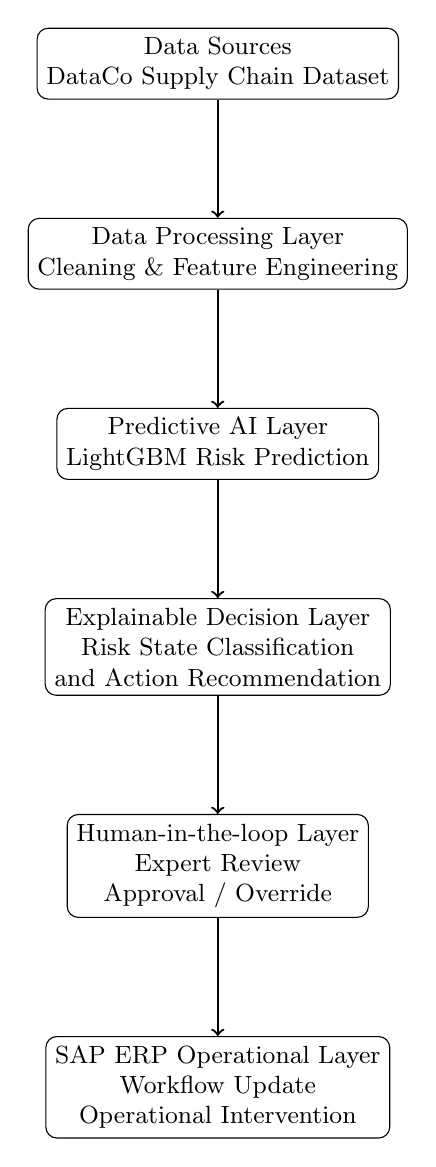
\begin{tikzpicture}[
node distance=1.5cm,
every node/.style={
    draw,
    rounded corners,
    align=center,
    minimum width=3.2cm,
    minimum height=0.9cm,
    font=\small
},
arrow/.style={->, thick}
]

\node (data) {
Data Sources\\
DataCo Supply Chain Dataset
};

\node (process) [below=of data] {
Data Processing Layer\\
Cleaning \& Feature Engineering
};

\node (ai) [below=of process] {
Predictive AI Layer\\
LightGBM Risk Prediction
};

\node (decision) [below=of ai] {
Explainable Decision Layer\\
Risk State Classification\\
and Action Recommendation
};

\node (human) [below=of decision] {
Human-in-the-loop Layer\\
Expert Review\\
Approval / Override
};

\node (sap) [below=of human] {
SAP ERP Operational Layer\\
Workflow Update\\
Operational Intervention
};

\draw[arrow] (data) -- (process);
\draw[arrow] (process) -- (ai);
\draw[arrow] (ai) -- (decision);
\draw[arrow] (decision) -- (human);
\draw[arrow] (human) -- (sap);

\end{tikzpicture}
\caption{Explainable human-in-the-loop AI decision layer workflow for SAP-oriented workflow integration.}
\label{fig:decision_pipeline}
\end{figure}

The predictive model estimates the probability of late delivery, while the decision layer transforms probabilistic outputs into actionable operational states. The resulting decisions are evaluated from workflow and economic perspectives. The framework is designed as a decision-support layer that complements enterprise processes rather than replacing human operational control.

The proposed SAP-oriented architecture is presented in Fig.~\ref{fig:sap_architecture}.

\begin{figure}[htbp]
\centering

\includegraphics[width=0.9\linewidth]{figures/sap_architecture_diagram.pdf}
\caption{Proposed SAP-oriented AI decision layer architecture.}
\label{fig:sap_architecture}
\end{figure}

\subsection{Data Preparation and Process Analysis}

The empirical analysis uses the DataCo Supply Chain dataset containing 180,519 order-level observations. The target variable is \texttt{Late\_delivery\_risk}, representing the binary late-delivery outcome.

The analysis examines operational variables including shipping mode, market, customer segment, order region, order-item quantity, product price, and related logistics attributes.

Categorical variables are encoded through a reproducible preprocessing pipeline, while numerical variables are retained in numerical form. Variables that directly encode the target outcome or introduce information leakage are excluded from predictive modeling.

The resulting feature matrix is represented as:

\[
X \in \mathbb{R}^{n \times p},
\]

where $n$ denotes the number of observations and $p$ the number of predictive variables. The target vector is:

\[
y \in \{0,1\}^{n}.
\]


\subsection{Process Capability Baseline}

Process capability analysis is used as a statistical baseline for historical process performance. Let the quality characteristic $X$ have process mean $\mu$ and standard deviation $\sigma$, with lower and upper specification limits $LSL$ and $USL$.

The capability index is:

\begin{equation}
C_{pk} =
\min\left(
\frac{USL-\mu}{3\sigma},
\frac{\mu-LSL}{3\sigma}
\right).
\end{equation}

The capability assessment provides a process-level diagnostic against which subsequent predictive analysis can be interpreted. A conventional threshold of $C_{pk}<1.33$ is treated as an indication of insufficient process capability.

Process capability is therefore used as a baseline diagnostic rather than as the predictive decision mechanism.


\subsection{Predictive Model Development}

Five supervised learning approaches are evaluated:

\begin{enumerate}
    \item Logistic Regression;
    \item Classification and Regression Trees (CART);
    \item Random Forest;
    \item XGBoost;
    \item LightGBM.
\end{enumerate}

For each model, the objective is to estimate:

\[
\hat{p}_i=P(Y_i=1\mid X_i),
\]

where $\hat{p}_i$ denotes the predicted probability that observation $i$ will experience late delivery.

Cross-validation is used to estimate predictive stability across data partitions. ROC-AUC is used as the principal discrimination metric because it evaluates ranking performance independently of a fixed classification threshold.

CART is additionally considered as an interpretable baseline model because its tree structure provides explicit decision rules. At node $t$, class impurity is measured using the Gini impurity:

\begin{equation}
I(t)=1-\sum_{i=1}^{C}p_i^2,
\end{equation}

where $p_i$ denotes the proportion of observations belonging to class $i$.
\subsection{Probability Calibration}

Since the proposed decision layer relies on predicted probabilities rather than only binary classifications, probability calibration is evaluated independently from predictive discrimination.

The Brier Score is used to measure the accuracy of probabilistic predictions:

\begin{equation}
BS=
\frac{1}{N}
\sum_{i=1}^{N}
(\hat{p}_i-y_i)^2,
\end{equation}

where $\hat{p}_i$ represents the predicted probability and $y_i$ denotes the observed outcome.

Expected Calibration Error (ECE) is calculated by partitioning predictions into $B$ probability bins:

\begin{equation}
ECE=
\sum_{b=1}^{B}
\frac{|S_b|}{N}
\left|
\operatorname{acc}(S_b)
-
\operatorname{conf}(S_b)
\right|.
\end{equation}

Calibration analysis evaluates whether predicted risk probabilities correspond consistently with observed late-delivery frequencies. This step is essential because operational decisions based on probability thresholds require reliable risk estimation rather than discrimination performance alone.


\subsection{Cost-Sensitive Decision Evaluation}

The economic evaluation investigates whether risk-based interventions provide measurable operational benefit under different cost assumptions.

For each observation $i$, the baseline expected cost without intervention is defined as:

\begin{equation}
C_{\mathrm{baseline},i}
=
\hat{p}_i C_L,
\end{equation}

where $C_L$ represents the assumed cost associated with a late-delivery event.

When an intervention is applied, the expected cost is modified by considering both residual late-delivery impact and intervention expenditure:

\begin{equation}
C_{\mathrm{decision},i}
=
C_{\mathrm{residual},i}
+
C_I I_i,
\end{equation}

where $C_I$ denotes the intervention cost and $I_i$ is a binary intervention indicator.

The total economic saving is calculated as:

\begin{equation}
S=
C_{\mathrm{baseline}}
-
C_{\mathrm{decision}}.
\end{equation}

The corresponding saving rate is:

\begin{equation}
SR=
\frac{S}{C_{\mathrm{baseline}}}.
\end{equation}

A positive value of $S$ indicates that the evaluated intervention policy provides economic benefit under the assumed cost configuration. The framework therefore avoids assuming that every predicted high-risk case should automatically trigger intervention.


\subsection{Cost Sensitivity and Break-Even Analysis}

Because economic outcomes depend strongly on operational cost assumptions, sensitivity analysis is performed across multiple combinations of late-delivery and intervention costs.

For each evaluated scenario, the decision policy is considered economically beneficial when:

\[
C_{\mathrm{decision}}
<
C_{\mathrm{baseline}}.
\]

The break-even intervention cost is defined as the maximum intervention cost for which:

\[
C_{\mathrm{decision}}
\leq
C_{\mathrm{baseline}}.
\]

This analysis identifies the economic boundary beyond which intervention is no longer justified and provides a practical mechanism for adapting the decision layer to organization-specific cost structures.

\begin{figure}[htbp]
\centering
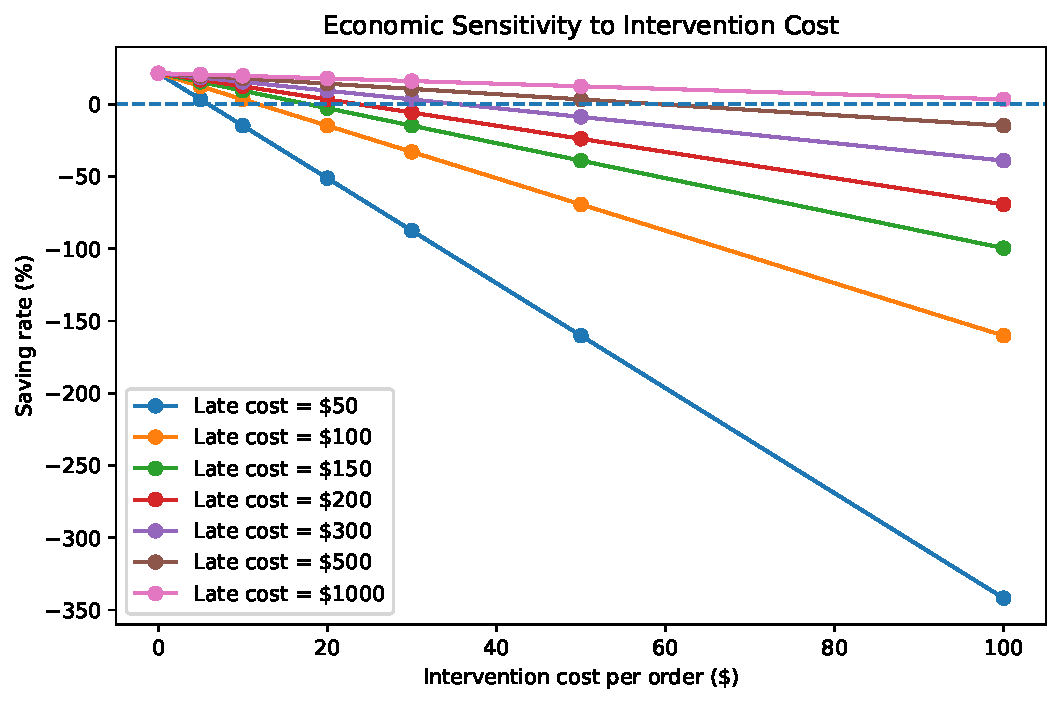
\includegraphics[width=0.85\linewidth]{../results/cost_sensitivity.pdf}
\caption{Cost sensitivity analysis of intervention scenarios.}
\label{fig:cost_sensitivity}
\end{figure}


\subsection{Human-in-the-Loop Decision Process}

The proposed framework incorporates human oversight as a decision-control mechanism for cases requiring additional operational assessment.

The decision process is represented as:

\[
\mathrm{Prediction}
\rightarrow
\mathrm{Risk\ Assessment}
\rightarrow
\mathrm{Operational\ Action}
\rightarrow
\mathrm{Human\ Review}
\rightarrow
\mathrm{Final\ Decision}.
\]

LOW-risk observations are assigned to standard automated processing, whereas MEDIUM- and HIGH-risk observations are considered candidates for human review.

The human-in-the-loop component is evaluated by measuring the number and proportion of observations routed for additional review. This provides an operational indicator of human involvement within the decision architecture.


\subsection{SAP-Oriented Workflow Integration}

The decision layer is mapped into an SAP-oriented workflow representation to demonstrate how predictive outputs can be transformed into enterprise actions.

The implementation represents a workflow simulation and does not claim direct production SAP deployment. The objective is to demonstrate the logical integration pathway between predictive analytics and enterprise workflow execution.

The architecture consists of five logical layers:

\begin{enumerate}
    \item logistics and operational data sources;
    \item machine-learning prediction layer;
    \item risk assessment and decision layer;
    \item human-review control layer;
    \item SAP-oriented workflow and action layer.
\end{enumerate}

Each processed observation is transformed into a structured decision record containing:

\begin{itemize}
    \item predicted late-delivery probability;
    \item operational risk category;
    \item recommended action;
    \item workflow state;
    \item human-review requirement;
    \item final decision status.
\end{itemize}

An audit record is maintained to support traceability, reproducibility, and future integration with enterprise governance mechanisms.


\subsection{End-to-End Evaluation}

The complete framework is evaluated through representative workflow cases covering LOW, MEDIUM, and HIGH-risk scenarios.

For each evaluated case, the framework records:

\[
\left\{
\hat{p},
R,
A,
H,
W,
F,
C_{\mathrm{baseline}},
C_{\mathrm{decision}}
\right\},
\]

where:

\begin{itemize}
    \item $\hat{p}$ represents the predicted probability;
    \item $R$ represents the operational risk category;
    \item $A$ represents the recommended operational action;
    \item $H$ represents the human-intervention state;
    \item $W$ represents the workflow status;
    \item $F$ represents the final decision outcome.
\end{itemize}

The final validation stage verifies the consistency between predictive outputs, operational decisions, workflow execution, and economic evaluation.

% ============================================================
\section{Results and Discussion}
% ============================================================

\subsection{Baseline Statistical Assessment}

The DataCo Supply Chain dataset contains 180,519 operational records covering multiple logistics attributes, including shipping mode, market, order region, product price, order quantity, and delivery-related variables.

The target variable, \textit{Late\_delivery\_risk}, represents the binary outcome indicating whether a delivery was classified as late.

Descriptive analysis was conducted to characterize the historical logistics process behavior and identify variations in delivery outcomes across different operational conditions. Categorical relationships were examined using contingency analysis and chi-square testing, while risk-group delivery performance was evaluated in subsequent decision-layer analyses.

The baseline assessment provides the statistical context for transitioning from retrospective process evaluation toward transaction-level probabilistic risk estimation.

\subsection{Predictive Model Performance}

Five supervised learning approaches were evaluated: CART, Logistic Regression, Random Forest, XGBoost, and LightGBM.

Random Forest achieved the highest mean cross-validated ROC-AUC:

\[
ROC\text{-}AUC = 0.7311,
\qquad
SD=0.0026.
\]

CART achieved a ROC-AUC of 0.7300, Logistic Regression 0.7299, XGBoost 0.7303, while LightGBM achieved a comparable performance level.

The evaluated models demonstrated moderate predictive discrimination. The relatively small differences among classifiers indicate that the operational value of the proposed framework does not rely exclusively on selecting the highest-performing predictive model. Instead, the framework focuses on transforming probabilistic predictions into interpretable risk categories, operational actions, human-review states, workflow execution, and economically evaluated decisions.

For subsequent decision-layer analysis, LightGBM was selected as the operational prediction model due to its competitive predictive performance and suitability for feature interpretation through importance analysis.

\begin{table}[htbp]
\centering
\caption{Predictive Model Performance}
\label{tab:model_performance}
\resizebox{\columnwidth}{!}{
\begin{tabular}{lllrrrr}
\toprule
analysis & model & metric & mean & std & min & max \\
\midrule
Cross-Validation & Random Forest & ROC-AUC & 0.7311 & 0.0026 & 0.7275 & 0.7357 \\
Cross-Validation & CART & ROC-AUC & 0.7300 & 0.0026 & 0.7251 & 0.7347 \\
Cross-Validation & Logistic Regression & ROC-AUC & 0.7299 & 0.0030 & 0.7264 & 0.7373 \\
Gradient Boosting & XGBoost & ROC-AUC & 0.7303 & 0.0041 & NaN & NaN \\
Gradient Boosting & XGBoost & PR-AUC & 0.8008 & 0.0032 & NaN & NaN \\
Gradient Boosting & LightGBM & ROC-AUC & 0.7300 & 0.0044 & NaN & NaN \\
Gradient Boosting & LightGBM & PR-AUC & 0.8005 & 0.0035 & NaN & NaN \\
Random Seed Robustness & Logistic Regression & ROC-AUC & 0.7296 & 0.0003 & 0.7291 & 0.7300 \\
Random Seed Robustness & CART & ROC-AUC & 0.7300 & 0.0004 & 0.7296 & 0.7304 \\
Random Seed Robustness & Random Forest & ROC-AUC & 0.7310 & 0.0003 & 0.7305 & 0.7313 \\
\bottomrule
\end{tabular}
}
\end{table}

\begin{figure}[htbp]
\centering
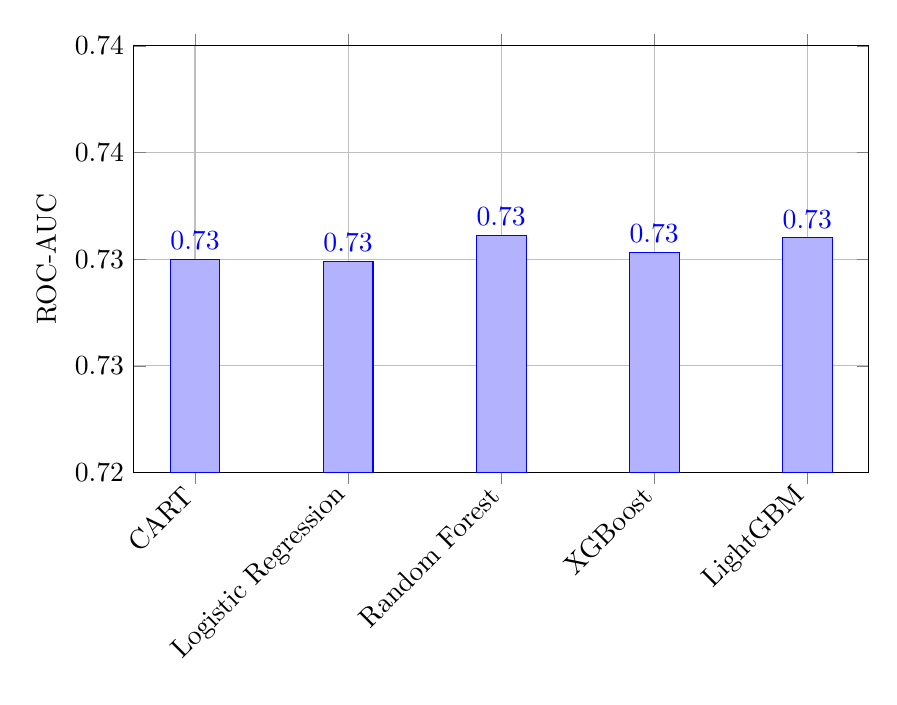
\begin{tikzpicture}
\begin{axis}[
    ybar,
    width=0.9\linewidth,
    height=7cm,
    ylabel={ROC-AUC},
    symbolic x coords={
        CART,
        Logistic Regression,
        Random Forest,
        XGBoost,
        LightGBM
    },
    xtick=data,
    ymin=0.72,
    ymax=0.74,
    nodes near coords,
    nodes near coords align={vertical},
    x tick label style={
        rotate=45,
        anchor=east
    },
    bar width=18pt,
    grid=major
]

\addplot coordinates {
    (CART,0.7300)
    (Logistic Regression,0.7299)
    (Random Forest,0.7311)
    (XGBoost,0.7303)
    (LightGBM,0.7310)
};

\end{axis}
\end{tikzpicture}
\caption{Comparison of predictive model performance using ROC-AUC.}
\label{fig:model_comparison}
\end{figure}

\begin{figure}[htbp]
\centering
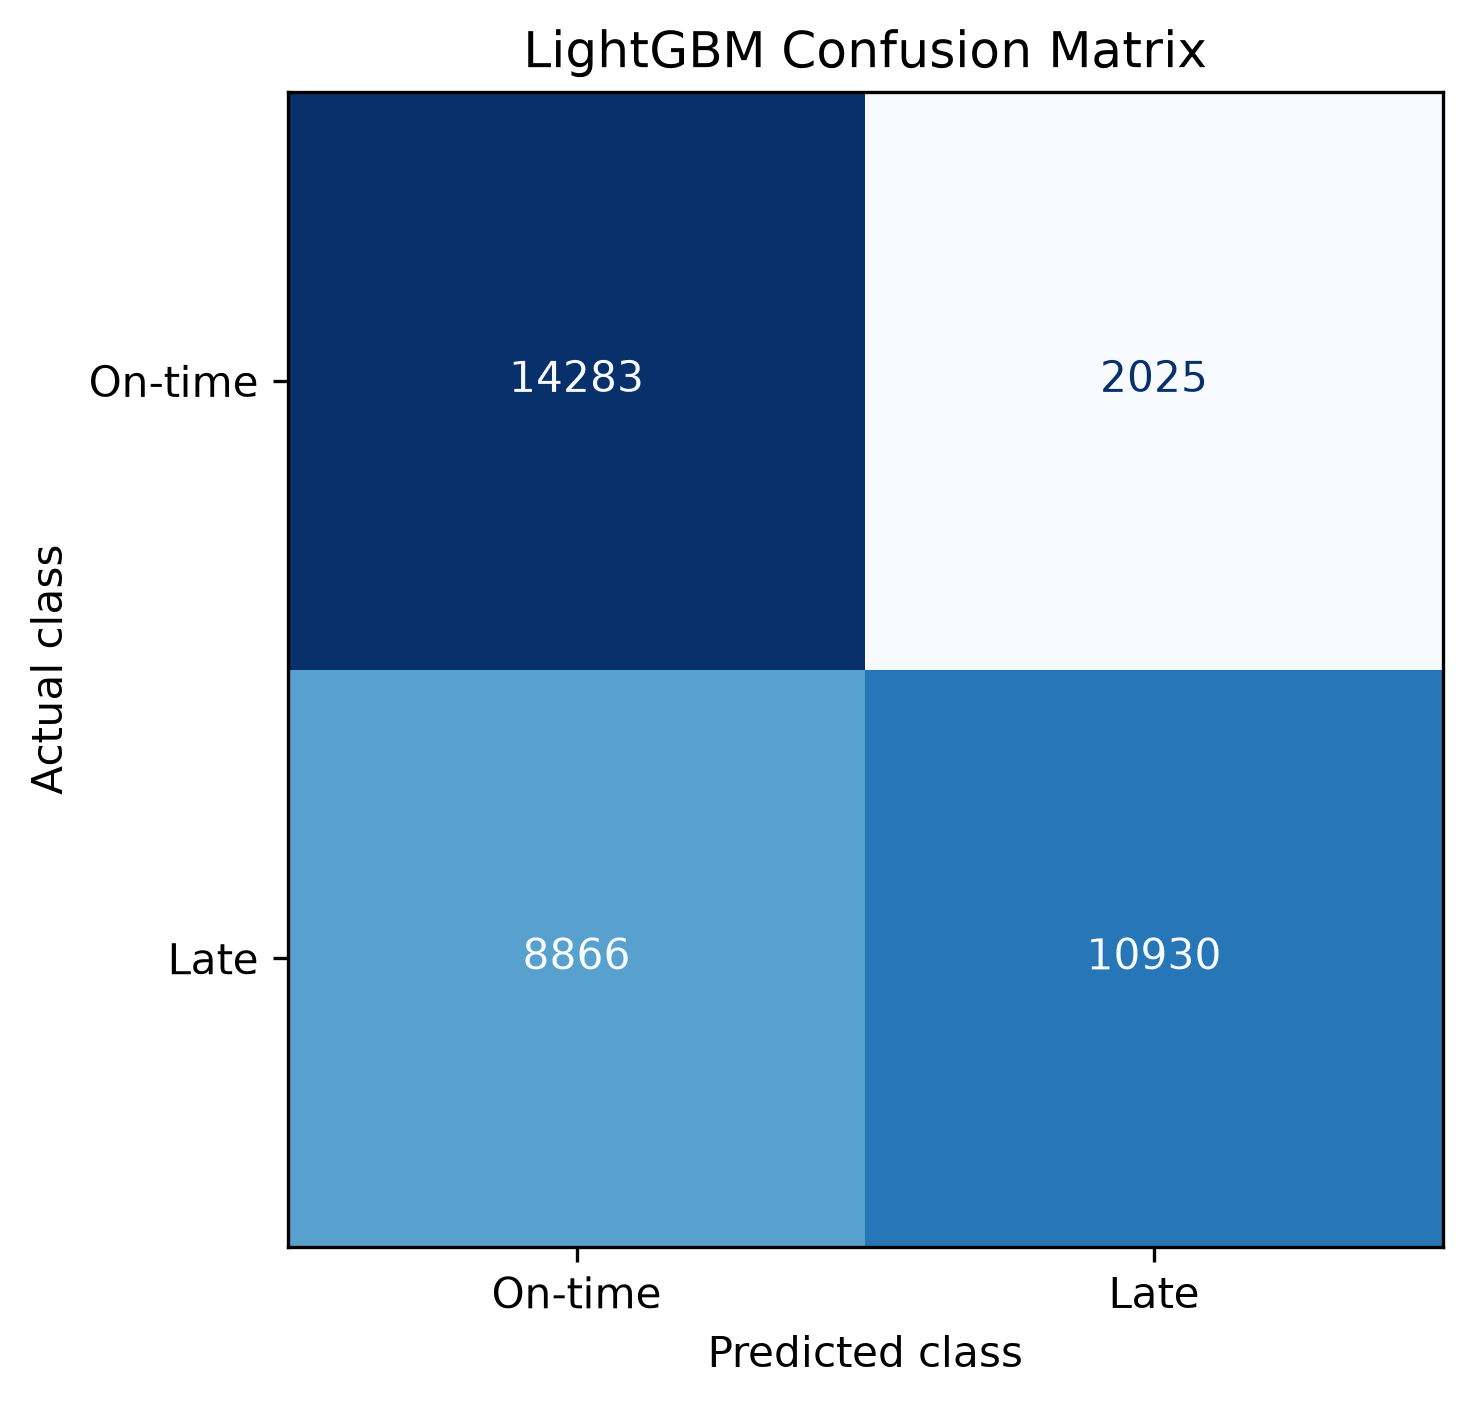
\includegraphics[width=0.65\linewidth]{../results/confusion_matrix.png}
\caption{Confusion matrix of the selected LightGBM classifier on the held-out test set.}
\label{fig:confusion_matrix}
\end{figure}

\begin{figure}[htbp]
\centering
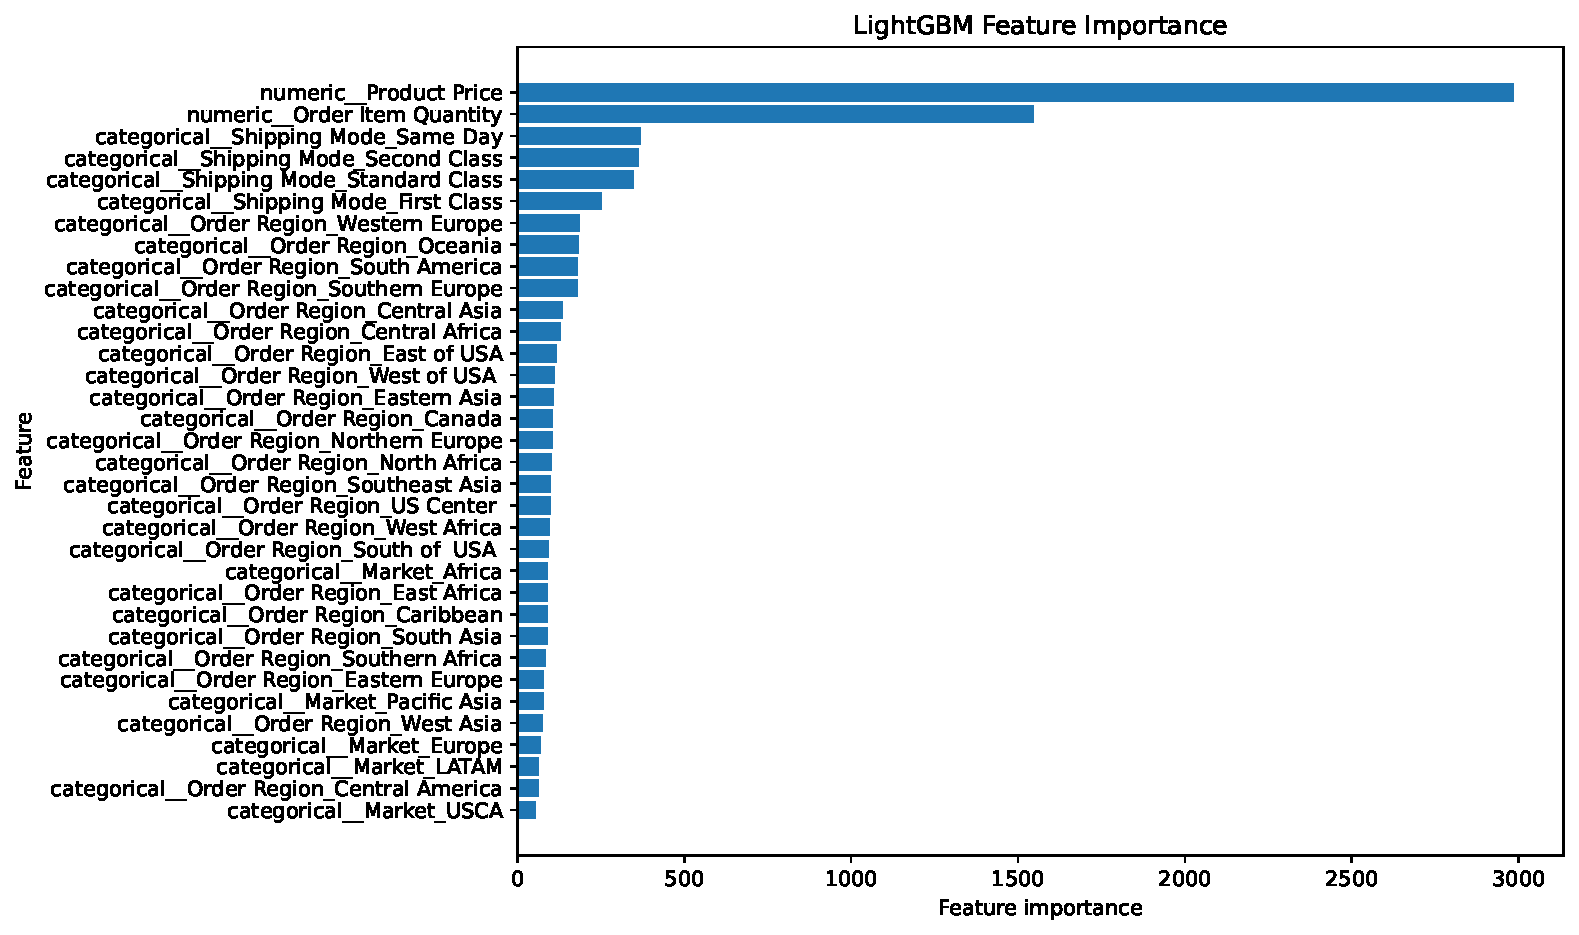
\includegraphics[width=0.85\textwidth]{../results/feature_importance.pdf}
\caption{Feature importance analysis of the selected LightGBM classifier for late-delivery risk prediction.}
\label{fig:feature_importance}
\end{figure}

\subsection{Risk Stratification}

Predicted probabilities generated by the selected predictive model were transformed into three operational risk categories: LOW, MEDIUM, and HIGH.

The observed late-delivery rates within each risk category were:

\[
\begin{aligned}
P(Y=1\mid LOW) &= 0.3855,\\
P(Y=1\mid MEDIUM) &= 0.6789,\\
P(Y=1\mid HIGH) &= 0.9320.
\end{aligned}
\]

The difference between HIGH and LOW risk groups was an absolute risk gap of 0.5465, corresponding to 54.65 percentage points.

The observed late-delivery rate increased monotonically across the risk categories. Furthermore, the association between risk level and observed late-delivery outcome was statistically significant ($p<0.001$), indicating that the generated risk states provide meaningful operational differentiation.

These results demonstrate that probabilistic predictions can be transformed into interpretable risk categories suitable for downstream decision-making.

\begin{table}[htbp]
\centering
\caption{Risk Stratification Effectiveness}
\label{tab:risk_effectiveness}
\begin{tabular}{lcc}
\toprule
Risk Level & Late-Delivery Rate & Decision State \\
\midrule
LOW & 38.55\% & Standard Process \\
MEDIUM & 67.89\% & Shipping Plan Review \\
HIGH & 93.20\% & Order Priority Review \\
\midrule
HIGH--LOW Gap & 54.65 percentage points & -- \\
\bottomrule
\end{tabular}
\end{table}

\begin{figure}[htbp]
\centering
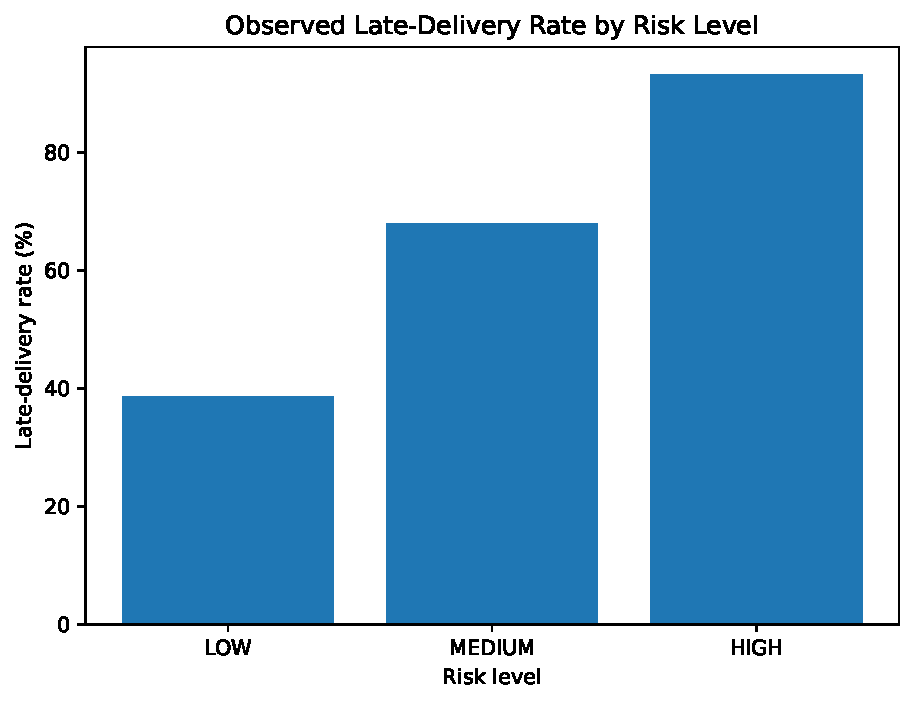
\includegraphics[width=0.85\linewidth]{../results/risk_effectiveness.pdf}
\caption{Observed late-delivery rates across operational risk categories.}
\label{fig:risk_effectiveness}
\end{figure}


\subsection{Probability Calibration}

Probability calibration was evaluated to assess the consistency between predicted probabilities and observed late-delivery outcomes. Two complementary metrics were used: the Brier Score and Expected Calibration Error (ECE).

For the selected LightGBM probability model, calibration evaluation on 36,104 held-out test observations produced:

\[
BS=0.1941,
\]

and:

\[
ECE=0.0046.
\]

The low ECE value indicates a small average difference between predicted confidence levels and observed event frequencies across calibration bins in the evaluated test set.

\begin{figure}[htbp]
\centering
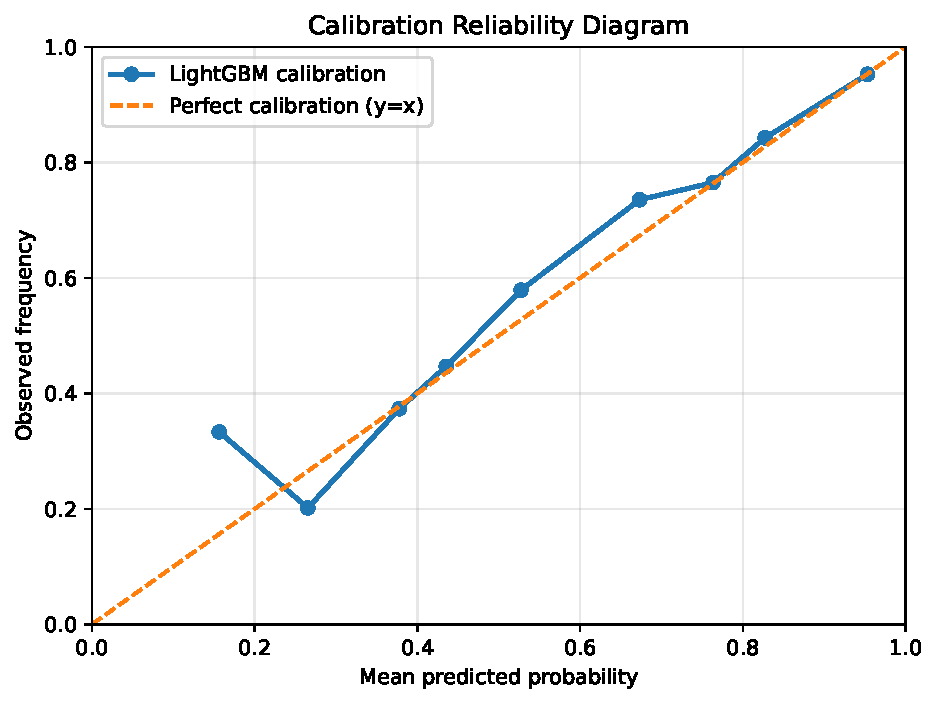
\includegraphics[width=0.8\linewidth]{../results/calibration_curve.pdf}
\caption{Probability calibration curve of the selected predictive model.}
\label{fig:calibration_curve}
\end{figure}

The calibration results indicate that the generated probability estimates exhibit reasonable agreement with observed outcomes, supporting their use as inputs for subsequent risk stratification and cost-sensitive decision analysis.

\begin{table}[htbp]
\centering
\caption{Probability Calibration Results}
\label{tab:calibration}
\resizebox{\columnwidth}{!}{
\begin{tabular}{rrrr}
\toprule
Bin & Mean Predicted Probability & Observed Frequency & Absolute Calibration Error \\
\midrule
1 & 0.1564 & 0.3333 & 0.1769 \\
2 & 0.2655 & 0.2017 & 0.0638 \\
3 & 0.3777 & 0.3734 & 0.0043 \\
4 & 0.4354 & 0.4467 & 0.0113 \\
5 & 0.5274 & 0.5789 & 0.0516 \\
6 & 0.6731 & 0.7353 & 0.0622 \\
7 & 0.7634 & 0.7650 & 0.0017 \\
8 & 0.8272 & 0.8424 & 0.0152 \\
9 & 0.9532 & 0.9527 & 0.0005 \\
\bottomrule
\end{tabular}
}
\end{table}

\subsection{SAP-Oriented Decision Layer}

The calibrated probability estimates were transformed into operational risk states and corresponding SAP-oriented workflow actions.

LOW-risk observations were assigned to:

\[
\texttt{SAP\_STANDARD\_PROCESS},
\]

MEDIUM-risk observations to:

\[
\texttt{SAP\_SHIPPING\_PLAN\_REVIEW},
\]

and HIGH-risk observations to:

\[
\texttt{SAP\_ORDER\_PRIORITY\_REVIEW}.
\]

The decision layer provides an explicit mapping between probabilistic risk estimation and operational workflow states. This separation ensures that predictive outputs are converted into interpretable actions rather than directly triggering automated operational changes.

The implementation represents an SAP-oriented workflow simulation for demonstrating decision integration concepts and does not claim a direct production SAP deployment.

\subsection{Human-in-the-Loop Decision Control}

The human-in-the-loop mechanism represents an explicit decision-control stage for observations requiring additional operational assessment.

Across 36,104 evaluated observations, 12,672 were assigned to human-in-the-loop review decisions, corresponding to:

\[
HITL\ Rate = 35.10\%.
\]

This result indicates that human involvement was modeled as an explicit operational decision state rather than being considered only as a conceptual requirement.

\begin{figure}[htbp]
\centering
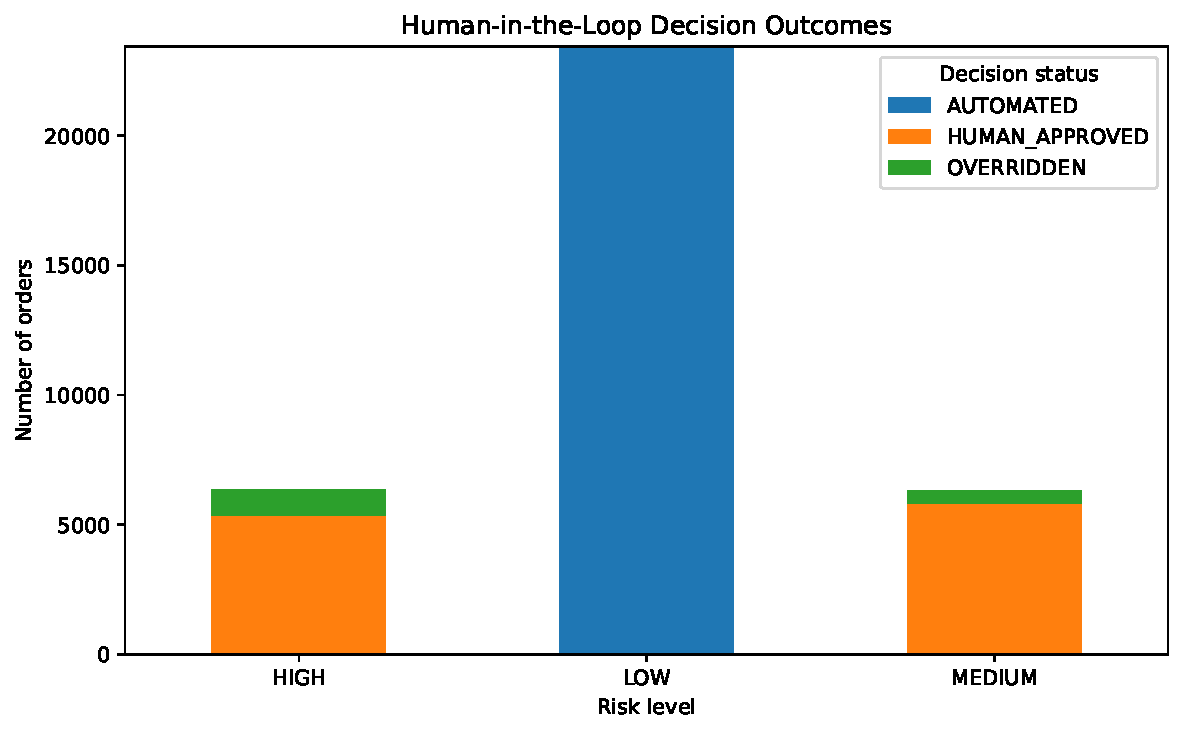
\includegraphics[width=0.85\linewidth]{../results/human_in_the_loop_flow.pdf}
\caption{Human-in-the-loop decision outcomes across risk levels.}
\label{fig:human_in_the_loop}
\end{figure}

The workflow simulation was further validated using representative LOW, MEDIUM, and HIGH-risk cases. All evaluated test cases successfully completed the simulated workflow sequence and reached a final approved state.

\subsection{Economic Impact and Sensitivity Analysis}

Economic evaluation was conducted to assess whether the proposed decision layer can reduce the expected cost associated with late deliveries under the defined cost assumptions.

Under the primary evaluated cost configuration, the baseline expected cost was:

\[
C_{\mathrm{baseline}}=\$9,897,690.45.
\]

The corresponding expected cost after applying the decision policy was:

\[
C_{\mathrm{decision}}=\$9,561,435.12.
\]

The resulting cost saving was:

\[
S=\$336,255.34,
\]

corresponding to:

\[
SR=3.40\%.
\]

To evaluate robustness against cost assumptions, 49 combinations of late-delivery and intervention costs were examined. Positive economic benefit was obtained in 30 of the evaluated scenarios.

These results indicate that the economic value of intervention depends on the relative relationship between late-delivery cost and intervention cost. Therefore, the framework does not assume that every high-risk prediction should automatically trigger intervention; instead, intervention decisions remain subject to cost-sensitive evaluation.

\begin{table}[htbp]
\centering
\caption{Economic Impact of the Decision Layer}
\label{tab:economic_impact}
\begin{tabular}{lr}
\toprule
Metric & Value \\
\midrule
Baseline Cost & \$9,897,690.45 \\
Decision-Layer Cost & \$9,561,435.12 \\
Cost Saving & \$336,255.34 \\
Saving Rate & 3.40\% \\
Beneficial Scenarios & 30/49 \\
\bottomrule
\end{tabular}
\end{table}

\begin{figure}[htbp]
\centering
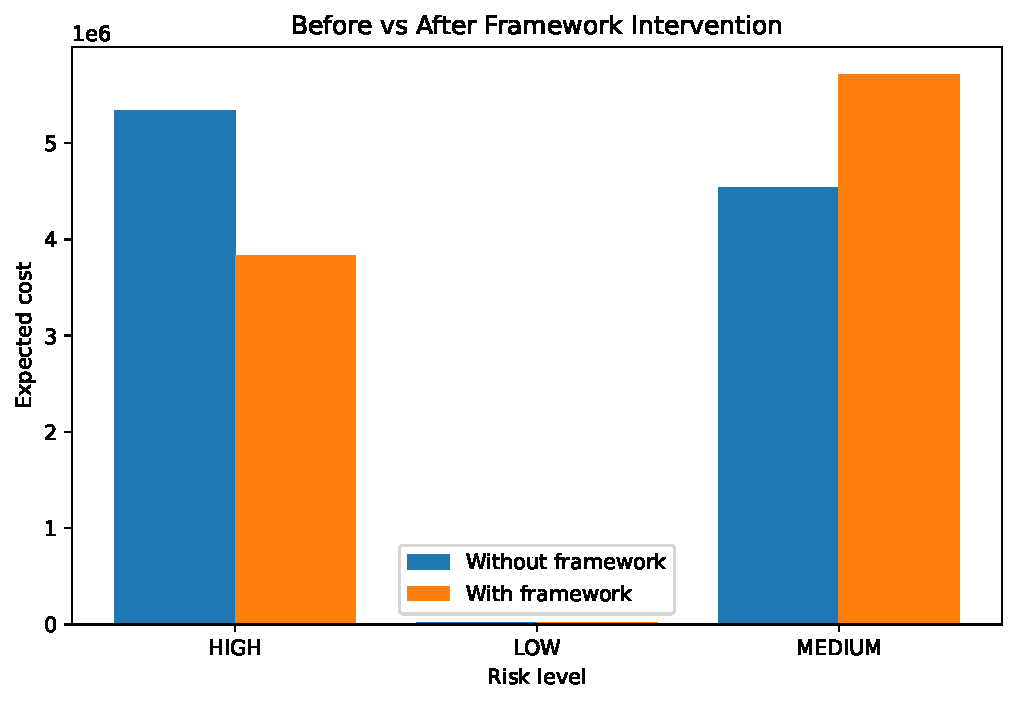
\includegraphics[width=0.85\linewidth]{../results/before_after_intervention.pdf}
\caption{Expected cost comparison before and after applying the decision policy.}
\label{fig:before_after}
\end{figure}

\subsection{Break-Even Analysis}

Break-even analysis was conducted to identify the maximum intervention cost at which the proposed decision policy maintains a non-negative economic benefit.

Seven late-delivery cost levels were evaluated, ranging from \$50 to \$1,000.

The corresponding break-even intervention costs increased with the assumed late-delivery cost, indicating that intervention feasibility depends on the relative cost relationship between avoiding late deliveries and applying corrective actions.

The break-even analysis therefore provides an operational decision boundary for identifying cost configurations under which intervention remains economically justified.

The resulting sensitivity surface illustrates the boundary between beneficial and non-beneficial intervention regions.

\begin{figure}[htbp] 
    \centering 
    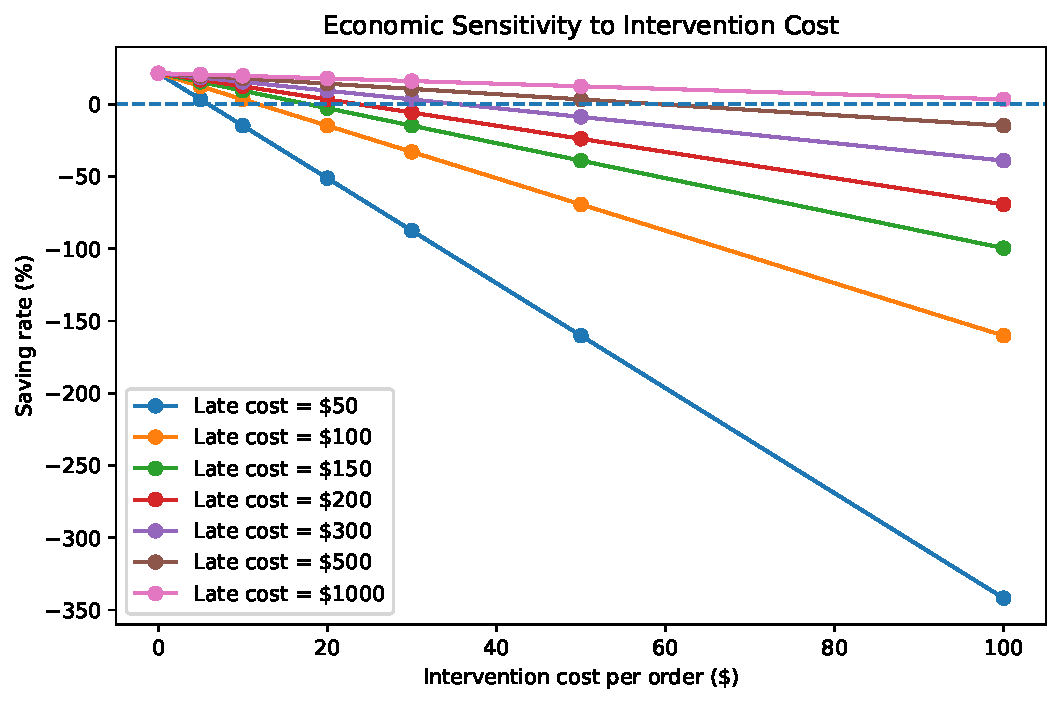
\includegraphics[width=0.85\linewidth]{../results/cost_sensitivity.pdf} 
    \caption{Cost sensitivity analysis.} 
    \label{fig:cost_sensitivity} 
\end{figure}

\begin{table}[htbp]
\centering
\caption{Economic Sensitivity Analysis}
\label{tab:economic_sensitivity}
\begin{tabular}{ccc}
\toprule
Scenario Group & Evaluated Scenarios & Beneficial Scenarios \\
\midrule
All Cost Combinations & 49 & 30 \\
\bottomrule
\end{tabular}
\end{table}

\subsection{SAP-Oriented Workflow Validation}

The decision layer was validated through a workflow simulation using representative LOW, MEDIUM, and HIGH-risk transaction cases.

The simulated workflow routed each case according to the generated risk state:

\[
\mathrm{LOW}
\rightarrow
\texttt{SAP\_STANDARD\_PROCESS},
\]

\[
\mathrm{MEDIUM}
\rightarrow
\texttt{SAP\_SHIPPING\_PLAN\_REVIEW},
\]

\[
\mathrm{HIGH}
\rightarrow
\texttt{SAP\_ORDER\_PRIORITY\_REVIEW}.
\]

All three representative test cases successfully completed the simulated workflow sequence and reached a final approved state.

The generated audit trail preserved the main decision attributes, including predicted probability, risk category, assigned SAP-oriented action, workflow status, human-review decision, and final outcome, supporting traceability and reproducibility of the decision process.
% ============================================================
\section{Discussion}
% ============================================================

The results indicate that the proposed framework extends beyond conventional predictive classification by establishing a connection between probabilistic risk estimation and operational decision processes.

The risk-stratification analysis demonstrated clear differentiation among LOW, MEDIUM, and HIGH operational risk categories based on observed late-delivery rates. In addition, the calibration analysis showed reasonable agreement between predicted probabilities and observed outcomes, supporting the use of probabilistic estimates as inputs for subsequent decision and economic evaluation layers.

The economic analysis provides an additional perspective on the practical value of predictive intervention. Under the primary evaluated cost configuration, the decision policy achieved a saving of \$336,255.34. However, only 30 out of 49 evaluated cost scenarios produced positive economic benefit, indicating that intervention effectiveness depends on the relative relationship between late-delivery costs and intervention costs rather than on risk prediction alone.

The break-even analysis further provides a mechanism for identifying cost conditions under which operational intervention remains economically justified. This prevents indiscriminate intervention by introducing economic constraints into the decision process.

From an enterprise-process perspective, the SAP-oriented workflow simulation demonstrates how predictive outputs can be transformed into traceable operational states, workflow actions, and selective human-review decisions. The audit trail generated by the framework supports transparency and reproducibility of the simulated decision process.

However, the study does not represent a production SAP deployment. The SAP component is implemented as a workflow-level simulation to demonstrate the operationalization of predictive decisions. Future industrial deployment would require integration with live enterprise transaction systems, real-time data streams, organizational authorization mechanisms, human feedback loops, and organization-specific economic parameters.
% ============================================================
\section{Conclusion}
% ============================================================

This study presented an end-to-end predictive decision framework for logistics risk management that integrates statistical process analysis, supervised machine learning, probability calibration, operational risk stratification, cost-sensitive decision evaluation, human-in-the-loop control, and SAP-oriented workflow simulation.

Using 180,519 logistics observations, the evaluated predictive models achieved moderate discrimination performance, with Random Forest obtaining the highest cross-validated ROC-AUC of 0.7311. The risk-stratification analysis demonstrated meaningful separation among operational risk categories, while calibration evaluation indicated that the generated probability estimates were sufficiently aligned with observed outcomes for use within downstream decision processes.

Under the primary evaluated cost configuration, the proposed decision policy achieved a cost saving of \$336,255.34, corresponding to a saving rate of 3.40\%. Sensitivity analysis further showed that 30 out of 49 evaluated cost scenarios resulted in positive economic benefit, highlighting the importance of incorporating cost considerations into predictive intervention decisions. The human-in-the-loop simulation represented human review as an explicit decision-control stage, with 35.10\% of evaluated observations routed for additional assessment.

The findings suggest that the primary contribution of the proposed framework is not limited to improving predictive performance, but rather to establishing a structured pathway that transforms predictive probabilities into interpretable risk states, operational workflows, human-review decisions, and economically evaluated actions.

Future research should investigate the framework using real-time enterprise data, production-level SAP system integration, adaptive human feedback mechanisms, and organization-specific cost models to evaluate scalability and practical deployment potential.
% ============================================================
% References
% ============================================================

\bibliographystyle{IEEEtran}
\bibliography{references}

\end{document}